\documentclass[10pt]{beamer}

\usetheme[progressbar=frametitle]{metropolis}
\usepackage{appendixnumberbeamer}

\usepackage{booktabs}
\usepackage{dsfont}
\usepackage[scale=2]{ccicons}
\usepackage{numprint}
\npthousandsep{\,}

\usepackage{pgfplots}
\usepgfplotslibrary{dateplot}

\usepackage{xspace}
\newcommand{\themename}{\textbf{\textsc{metropolis}}\xspace}

\title{Games, norms and obligations}
%???
%\subtitle{An introduction}

% \date{\today}
\date{}
\author{Josua Potschien, Chris Venn}
% \institute{Center for modern beamer themes}
%\titlegraphic{\hfill\includegraphics[height=1.5cm]{logo.pdf}}
\metroset{background=dark}
\begin{document}
\maketitle


\begin{frame}{Table of contents}
  \setbeamertemplate{section in toc}[sections numbered]
  \tableofcontents%[hideallsubsections]
\end{frame}


\section[Normative Systems]{Normative Systems}
\begin{frame}[fragile]{Normative Systems}
\begin{definition}[Normative System]
A normative system is a description of good and
bad
\end{definition}
\begin{itemize}
    \item Hijacked plane
    \item Is is good or bad to shoot down the plane?
\end{itemize}
$\Rightarrow$ We need a more precise definition \\
There are some more definitions mentioned but all of them have their own flaws
\end{frame}

\begin{frame}[fragile]{Normative Systems}

General problems with the traditional approach of deontic logic:
\begin{itemize}
    \item Lawyers $\Rightarrow$ more classification problems
    \item Computer Scientists $\Rightarrow$ some problems are hard to specify as a norm
    \item And various other fields
\end{itemize}
\end{frame}


\section[Detachment]{Detachment}
\begin{frame}[fragile]{Detachment}
\begin{definition}
Detachment is a way to solve a problem in a normative system
with two conflicting rules or obligations. It is not possible to
use the detachment approach in every situation
\end{definition}
\begin{itemize}
    \item $O(\lnot kill)$ and $kill \to O(killgently)$
    \item Implies $killgently \to kill$
    \item Detachment can solve this paradox
    \item Consider $O(Q|P)$ as $Q$ ought to be the case given $P$
    \item Mistake: Conclude $O(Q)$ from $O(Q|P)$ and $P$
    \item With detachment we only conclude $O(Q)$ from $O(Q|P)$, if  $O(P)$ is given
\end{itemize}
\end{frame}

\section[Violation Games]{Violation Games}
\begin{frame}[fragile]{Violation Games}
\begin{definition}[Violation Games / Normative Systems]
Violation games are social interactions among
agents to determine whether violations have occurred, and
which sanctions will be imposed for such violations. A
normative system is a specification of violation games
\end{definition}

\end{frame}

\begin{frame}[fragile]{Violation Games}
\begin{figure}[!htb]
    \centering
    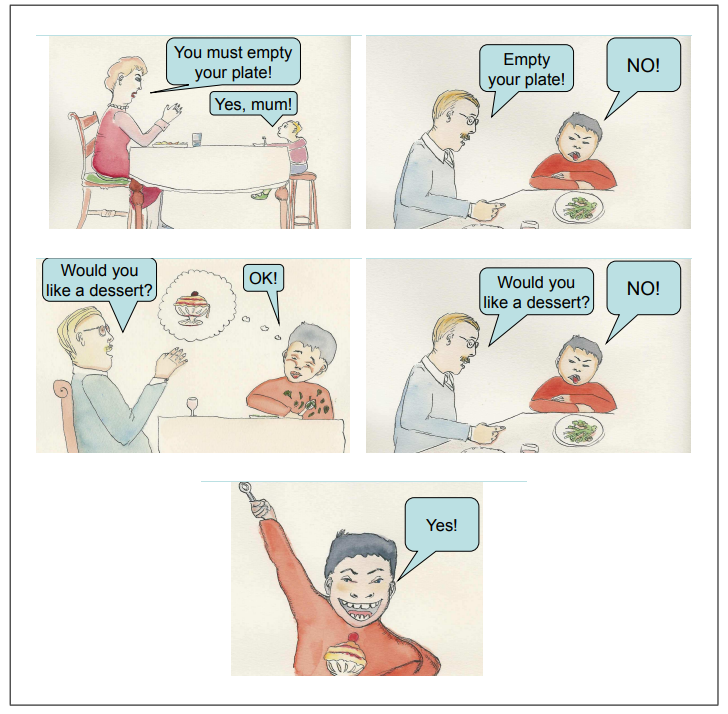
\includegraphics[scale=0.7]{1.png}
    \caption{Expectation, from [van der Torre, 2010]}
    \label{fig:my_label}
\end{figure}
\end{frame}

\begin{frame}[fragile]{Violation Games}
\begin{figure}[!htb]
    \centering
    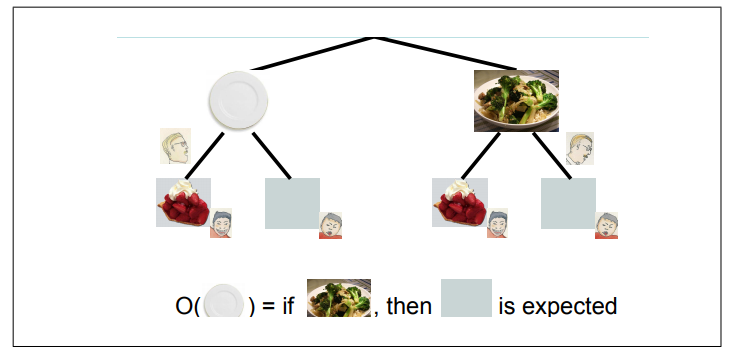
\includegraphics[scale=0.8]{2.png}
    \caption{Expectation, from [van der Torre, 2010]}
    \label{fig:my_label}
\end{figure}
\begin{itemize}
    \item $O(eatVegetables) = notEatingVegetables \to noDessert$
\end{itemize}
\end{frame}

\begin{frame}[fragile]{Violation Games}
\begin{figure}[!htb]
    \centering
    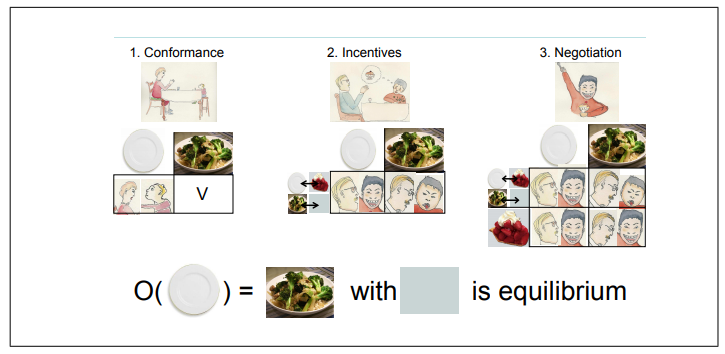
\includegraphics[scale=0.8]{3.png}
    \caption{Expectation, from [van der Torre, 2010]}
    \label{fig:my_label}
\end{figure}
\begin{itemize}
    \item $O(eatVegetables) = notEatingVegetables$ with $noDessert$ is an equilibrium
\end{itemize}
\end{frame}

\begin{frame}[fragile]{Violation Games}
We can separate the behaviour into different phases:\\
\begin{itemize}
    \item Phase 1: Son eats vegetables and violation does not occur
    \item Phase 2: Not eating vegetables is identified with absence of dessert
    \item Phase 3: As long as the norm is in force the son will believe to be sanctionized
    \item Phase 4: The norm is no longer in force
\end{itemize}
\end{frame}


\section[Norm Creation Games]{Norm Creation Games}
\begin{frame}[fragile]{Norm Creation Games}
\begin{definition}
Norm creation games are social interactions
among agents to determine which norms are in force, whether
norm violations have occurred, and which sanctions will
be imposed for such violations. A normative system is a
specification of norm creation games
\end{definition}
\begin{itemize}
    \item A pool with 100 bystanders and one child in the water\\
    $\to$ what are the norms/obligations?
    \item Consider mental modalities of each bystander
    \item The more you know about the situation the more you can say about the protocol that leads to the norm
\end{itemize}

\end{frame}

\section[Conclusion]{Conclusion}
\begin{frame}[fragile]{Conclusion}
\begin{itemize}
    \item Actions, mental modalities and permissions are important for violation games
    \item We can't use the violation games approach in every scenario (hijacked plane)
    \item Negotiation is an essential part to model a violation game
    \item Norm creation games have no practical use
    \item Trying to use game theory on the hijacked plane example leads to no solution
\end{itemize}
\end{frame}

\begin{frame}[fragile]{Conclusion}
 How can deontic logic be based
on both norm and detachment, as well as decision and game
theory?
\begin{itemize}
    \item Kind of impossible to model every moral dilemma
    \item Violation games itself are complex enough
    \item Detachment approach can be combined with hijacked plane example but also leads to no practical solution
    \item In our opinion it is not possible to combine norm, detachment and decision and game theory
\end{itemize}
\end{frame}

% ------- Sources ----------
\begin{frame}[fragile]{Sources}
\begin{itemize}
    \item https://en.wikipedia.org/wiki/Social\_norm
    \item L. van der Torre. Violation games: a new foundation for deontic logic.
Journal of Applied Non-Classical Logics, 20(4):457–477, 2010
    \item Gabriella Pigozzi, Leendert van der Torre. Multiagent Deontic Logic
and its Challenges from a Normative Systems Perspective
\end{itemize}
\end{frame}
% --------- END OF SLIDE -------------

\end{document}
